% !TEX program = xelatex
% coding=utf-8
\documentclass[14pt]{Bredelebeamer}
\usepackage{ctex}

\usepackage{multirow}
\usepackage{booktabs}
\usepackage{graphicx}
\usepackage{tikz}
\usepackage{epstopdf}
\usepackage{fontawesome}
\newfontfamily{\FA}{[FontAwesome.otf]}
\usetikzlibrary{arrows,decorations.markings}
\usetikzlibrary{decorations.pathreplacing}
\usetikzlibrary{calc}
 \setbeamerfont{title}{size=\LARGE}
 \setbeamerfont{subtitle}{size=\LARGE}
 \setbeamerfont{institute}{size=\large}
%%%%%%%%%%%%%%%%%%%%%%%%%%%%%%%%%%%%%%%%%%%%%%%%



\title[研究生开题答辩]{神经网络语言模型的性能优化研究}
\subtitle{On Optimization Perspective of Neural Language Model}
\institute[]{北京航空航天大学计算机学院研究生开题答辩}
\author[\href{mailto:nanjiang@buaa.edu.cn}{ \textit{nanjiang@buaa.edu.cn}}]{姜楠 (\href{mailto:nanjiang@buaa.edu.cn}{\textit{nanjiang@buaa.edu.cn}})}
\date{ 2016 年 12 月 20 日}
\subject{开题答辩}

\begin{document}

\begin{frame}
  \titlepage
\end{frame}

\begin{frame}{概览}
  \begin{columns}
    \begin{column}{.5\textwidth}
        \tableofcontents
    \end{column}
    \begin{column}{.5\textwidth}
      \begin{figure}
        \centering
        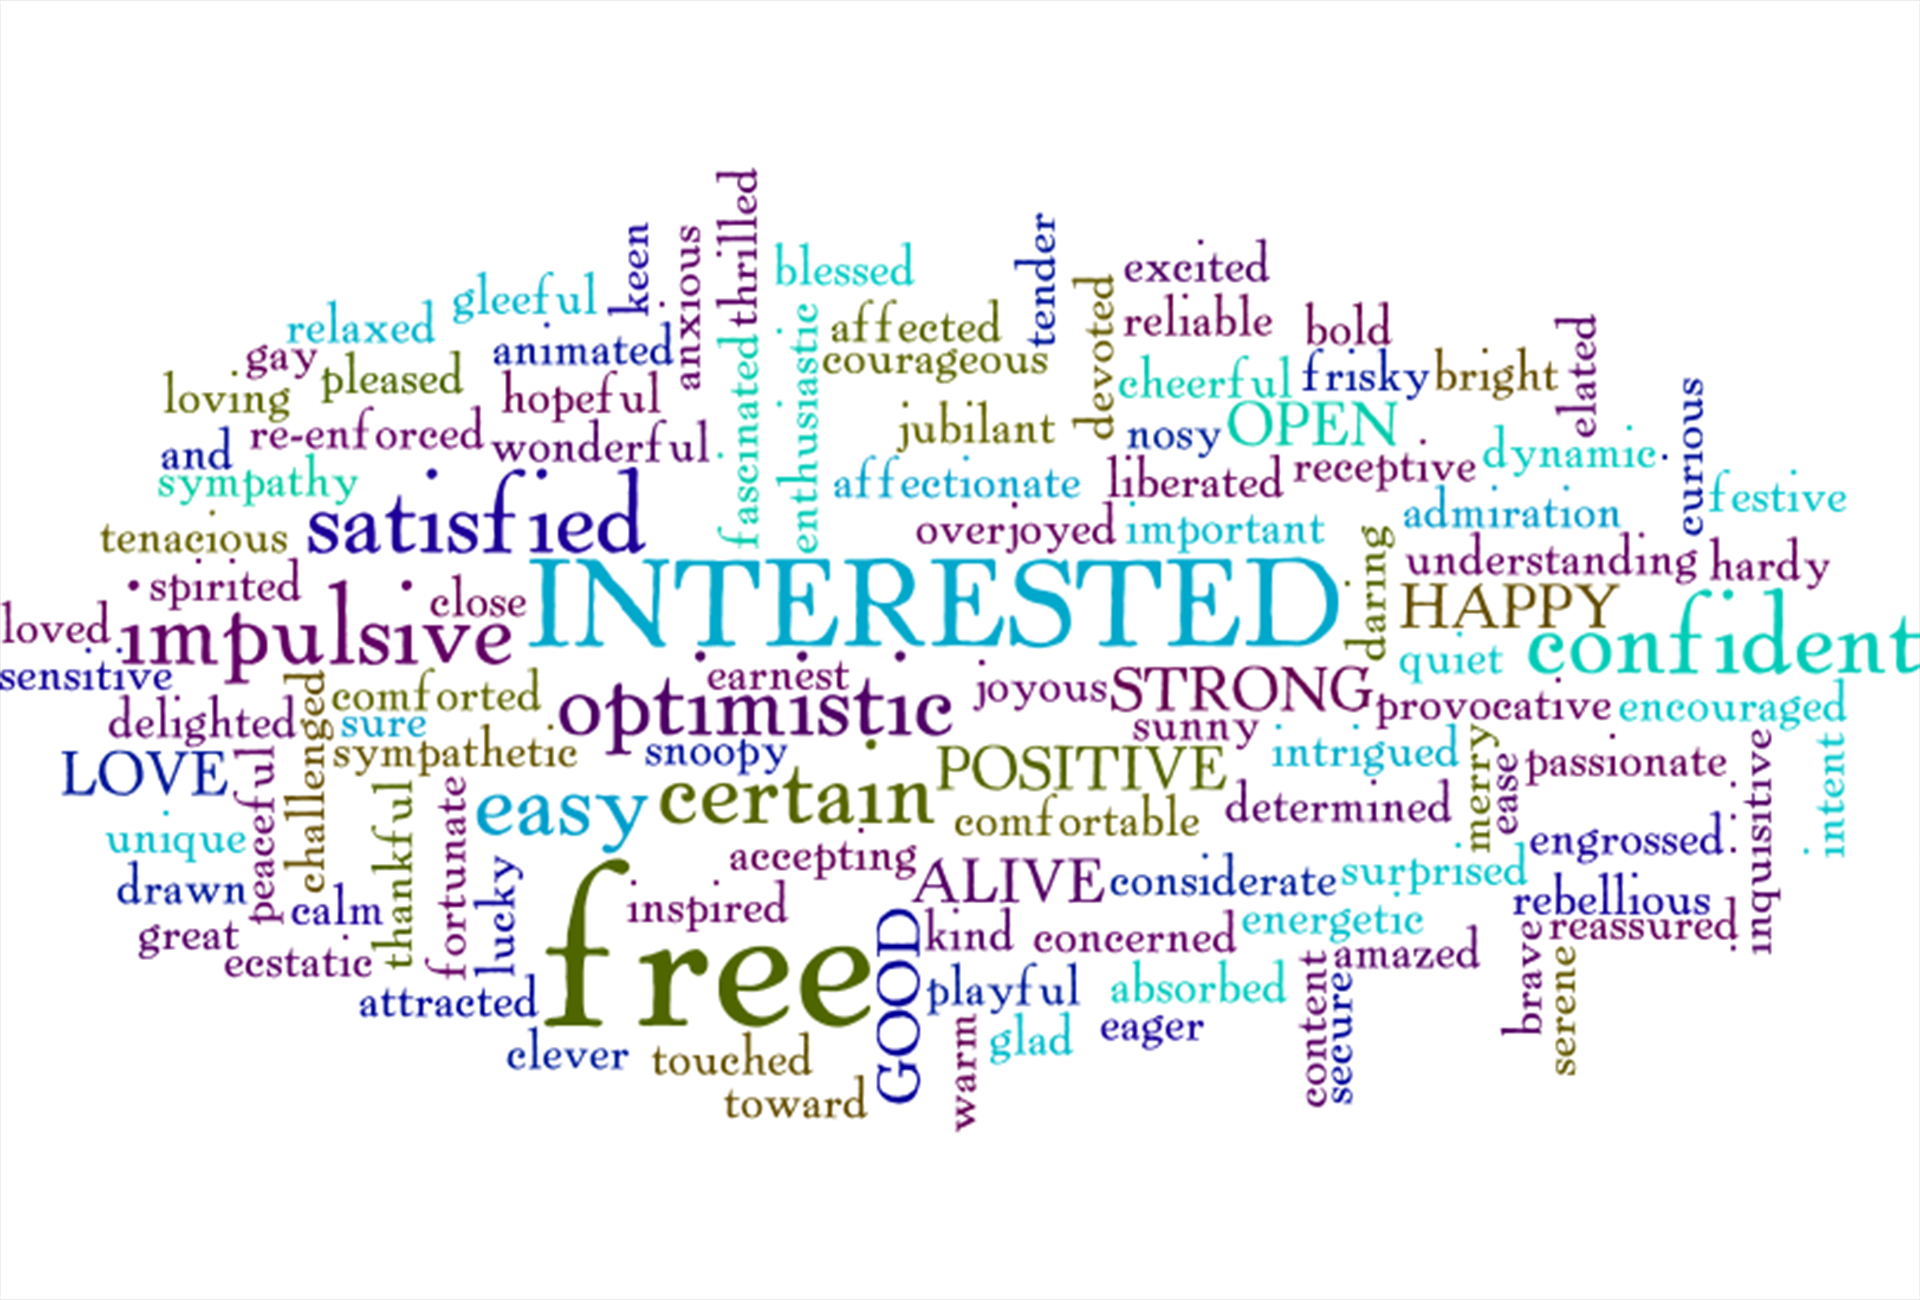
\includegraphics[width=1.\textwidth]{images/word-cloud.png}
      \end{figure}
    \end{column}
  \end{columns}
\end{frame}

\section{论文选题的背景与意义}
\begin{frame}{题目来源}
  论文题目《神经网络语言模型的性能优化研究》为自拟课题。
  \pause
  \begin{alertblock}{语言模型(Language Model)}
    \begin{itemize}
      \item 语言模型可以对一段文本的概率进行估计,对信息检索、机器翻译、语音识别等任务有着重要的作用
      \item 形式化讲,统计语言模型的作用是为一个长度为m的字符串确定一个概率分布$P(w_1;w_2; \cdots ;w_m)$,表示其存在的可能性
    \end{itemize}
  \end{alertblock}
  \pause
  \begin{block}<3->{神经网络}
    \begin{itemize}
      \item 人工神经网络是一个能够学习,能够总结归纳的系统,也就是说它能够通过已知数据的实验运用来学习和归纳总结。
      \item 与之不同的基于符号系统下的学习方法,它们也具有推理功能,只是它们是建立在逻辑演算法的基础上,也就是说它们之所以能够推理,基础是需要有一个推理演算法则的集合。
    \end{itemize}
  \end{block}
\end{frame}

\section{国内外研究现状及发展动态}
\begin{frame}{语言模型}

{\large
语言模型可以对一段文本的概率进行估计,对信息检索、机器翻译、语音识别等任务有着重要的作用。
形式化讲,统计语言模型的作用是为一个长度为m 的字符串确定一个概率分布$P(w_1;w_2;\cdots;w_m)$,表示其存在的可能性,其中$w_1$ 到$w_m$ 依次表示这段文
本中的各个词。一般在实际求解过程中,通常采用下式计算其概率值:
\begin{equation}
\label{equ:lm}
\begin{split}
P(w_1;w_2; \cdots;w_m) &= P(w_1) P(w_2|w_1) P(w_3|w_1;w_2)\cdots P(w_i | w_1;w_2;\cdots;w_{i-1}) \\
&\cdots P(w_m | w_1;w_2;\cdots;w_{m-1})
\end{split}
\end{equation}
在实践中,如果文本的长度较长,公式\ref{equ:lm}右部$\cdots P(w_m | w_1;w_2;\cdots;w_{m-1}) $ 的估算会非常困难。因此,研究者们提出使用一个简化模型:n 元模型(n-gram model)。在n 元模型中估算条件概率时,距离大于等于n 的上文词会被忽略,也就是对上述条件概率做了以下近似:
\begin{equation}
\label{equ:approx}
P(w_i | w_1;w_2;\cdots;w_{i-1})  \approx P(w_i | w_{i-(n-1)};\cdots;w_{i-1})
\end{equation}
}
\end{frame}


\subsection{隐写分析}

\begin{frame}{隐写分析}
  \begin{columns}
    \begin{column}{.25\textwidth}
      \begin{block}{}
        \begin{itemize}
          \item \alert<2>{视觉隐写分析}
          \item 结构隐写分析
          \item 统计隐写分析
          \item 学习隐写分析
        \end{itemize}
      \end{block}
    \end{column}
    \begin{column}{.7\textwidth}
      \pause
      \begin{figure}
        \centering
        \includegraphics[width=.95\textwidth]{images/lsb1}
      \end{figure}
    \end{column}
  \end{columns}
\end{frame}












\section{论文的研究内容及拟采取的技术方案}



\begin{frame}{循环神经网络}
	\begin{block}{样本集}
		容量为$N$的训练样本集$D = \left\{ {\left( {{{\mathbf{x}}_1},{y_1}} \right),\left( {{{\mathbf{x}}_2},{y_2}} \right), \ldots \left( {{{\mathbf{x}}_N},{y_N}} \right)} \right\}$
    \pause
		\begin{itemize}
			\item 特征向量${\mathbf{x}_i}$为图像块的特征
      \pause
			\item 标签$y_i \in \left\{ -1,1\right\}$为安全评估结果,在训练集中由隐写方法评估得到,在使用隐写系统时预测结果作为选择位置的参考指标
		\end{itemize}
	\end{block}
\pause
	\begin{alertblock}{SVM分类器}
			\begin{columns}
			\begin{column}{.5\textwidth}
		追求最大\alert<4>{“间隔”}的分类
		$$
		\begin{aligned}
		\mathop {\max }\limits_{{\mathbf{w}},b} & \quad\frac{2}{{\left\| {\alert<4>{\mathbf{w}}} \right\|}} \\
		s.t. &\quad {y_i}  \left( {{{\mathbf{w}}^T}{\mathbf{x_i}} + b} \right) \ge 1,i = 1,2, \ldots ,N
		\end{aligned}$$
			\end{column}
      \pause
					\begin{column}{.41\textwidth}
						过度拟合\&线性不可分
						\begin{itemize}
              \pause
							\item 核函数:变换特征空间至高维
              \pause
							\item 软间隔:以权重$C$容忍分类错误
						\end{itemize}
						\end{column}
		\end{columns}
	\end{alertblock}
\end{frame}






\subsection{拟采取的技术方案}
\begin{frame}{实验平台和设置}
	\begin{description}
		\item[Linux] 操作系统
		\item[R] 主要用于数据统计和图表处理
		\item[Python2.7] 使用的开发语言和开发环境
		\item[Theano] 主要的建模语言
	\end{description}
  \pause
	\begin{block}{}
		\begin{itemize}
			\item 同时还依赖于其他的处理脚本,需要对bash script和C/C++ 有足够的了解和掌握;
			\item GPU的设备是使用Titan X, 并且对应的CUDA版本为8.0(需要CUDNN/CUSPARSE等库的支持).
		\end{itemize}
	\end{block}
\end{frame}

\subsection{论文的研究内容}
\begin{frame}{SVM的训练}
	使用80组不同参数进行训练,得到的SVM在错误率方面的表现
\end{frame}

\section{论文研究计划}
\begin{frame}{时间安排}
	\begin{block}{}
\begin{itemize}
  \item 2016年12月 $\sim$ 2017年1月: 整理资料,学习研究语言模型的领域知识;
  \item 2017年2月$\sim$ 2017年4月: 研究学习深度学习模型的知识, 特别是循环神经网络的建模过程;
  \item 2017年5月$\sim$2017年7月: 调研并实现解决大词表问题的主要手段, 并实现基本代码框架;
  \item 2015年8月$\sim$2015年10月: 实验验证与完善;
  \item 2015年11月$\sim$2015年12月:资料整理和论文撰写.
\end{itemize}
    \end{block}
\end{frame}

\begin{frame}{Thanks}
	\centering
    谢谢各位老师和同学!请大家批评指正;

	论文中用到的全部源代码(包括本幻灯片),数据,图像,文档见:
	 {\faGithub~~\url{https://github.com/jiangnanHugo/Graduate_Design}}
\end{frame}

\end{document}
